\documentclass[tikz,border=2pt]{standalone}
\usepackage{amsmath,amssymb}
\usepackage{tikz}
\usetikzlibrary{arrows.meta}

\begin{document}
% At a constrained optimum the gradient of f is a multiple of the constraint gradient; the
% multiplier mu is that factor, and it also measures how fast the optimal value grows when
% the constraint level c is raised.
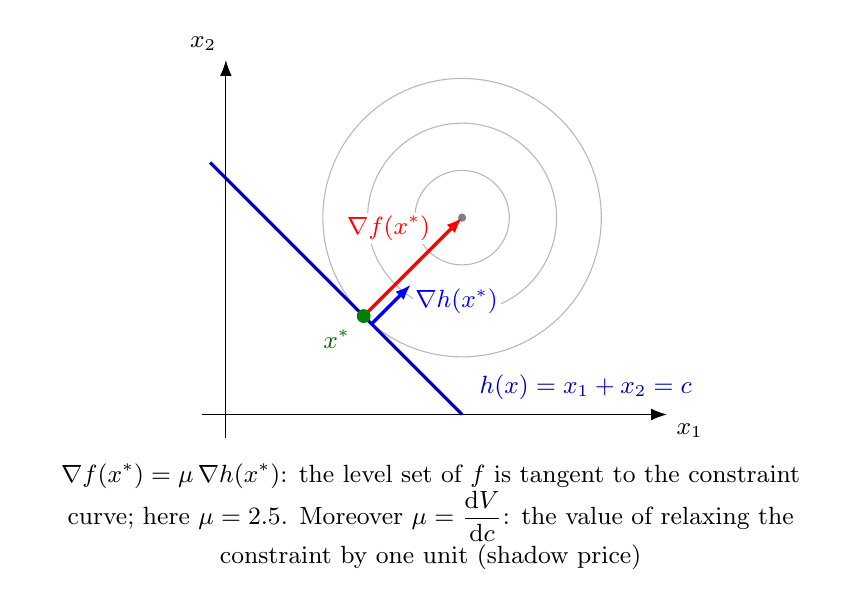
\begin{tikzpicture}[every node/.style={font=\small}, >={Latex[length=2mm]}, lab/.style={font=\small, fill=white, inner sep=1pt}]
	\foreach \r in {0.6,1.2,1.768} {\draw[gray!55] (3,2.5) circle (\r);}
	\fill[gray] (3,2.5) circle (1.5pt);
	\draw[->] (-0.3,0) -- (5.6,0) node[below right] {$x_1$};
	\draw[->] (0,-0.3) -- (0,4.5) node[above left] {$x_2$};
	\draw[blue!70!black, very thick] (3.0,0) -- (-0.2,3.2);
	\node[blue!70!black, anchor=south west, font=\small] at (3.1,0.06) {$h(x)=x_1+x_2=c$};
	\draw[->, red, very thick] (1.75,1.25) -- (3.0,2.5) node[pos=0.72, above left, lab] {$\nabla f(x^\ast)$};
	\draw[->, blue, very thick] (1.85,1.15) -- (2.35,1.65) node[below right, lab] {$\nabla h(x^\ast)$};
	\fill[green!50!black] (1.75,1.25) circle (2.5pt);
	\node[green!40!black, anchor=north east, font=\small] at (1.7,1.2) {$x^\ast$};
	\node[anchor=north, align=flush center, text width=10cm] at (2.6,-0.5) {$\nabla f(x^\ast)=\mu\,\nabla h(x^\ast)$: the level set of $f$ is tangent to the constraint curve; here $\mu=2.5$. Moreover $\mu=\dfrac{\mathrm dV}{\mathrm dc}$: the value of relaxing the constraint by one unit (shadow price)};
\end{tikzpicture}
\end{document}
